\documentclass[11pt]{extreport}

\input{settings}

\begin{document}

% Dla lepszej wydajności można w trakcie pisania zakomentować obydwa include
\begin{titlepage}

% Redu marginile
\newgeometry{left=2cm,right=2cm,bottom=1cm}

\begin{figure}[!htb]
    \centering
    \begin{minipage}[c]{0.2\textwidth}
        \centering
        
\includegraphics[width=0.7\linewidth]{images/loga/PK_logo.jpg}
    \end{minipage}
    \hfill
    \begin{minipage}{0.55\textwidth}
        \large
        \vspace{0.2cm}
        \fontsize{14pt}{16pt}\selectfont
        \begin{center}
            \textbf{POLITECHNIKA KRAKOWSKA \\ im. T. Kościuszki}
        \end{center}
        \begin{center}
                Wydział Inżynierii Elektrycznej i Komputerowej \\
                 \textbf{Katedra Automatyki i Informatyki E-1}
        \end{center}
    \end{minipage}
    \hfill
    \begin{minipage}[c]{0.2\textwidth}
    \centering
        
\includegraphics[width=0.7\linewidth]{images/loga/wm_logo.jpg}
    \end{minipage}
\end{figure}

\begin{flushleft}
\fontsize{14pt}{16pt}\selectfont
Kierunek studiów: Informatyka w inżynierii komputerowej \\
Specjalność: -
\end{flushleft}

\vspace{1cm}

\begin{center}
\fontsize{14pt}{16pt}\selectfont
STUDIA NIESTACJONARNE
\end{center}

\vspace{0.5cm}
\begin{center}
\fontsize{24pt}{26pt}\selectfont
\textbf{PRACA DYPLOMOWA} \\
\end{center}
\begin{center}
\fontsize{12pt}{14pt}\selectfont
INŻYNIERSKA
\end{center}
\vspace{0.5cm}
\begin{center}
\fontsize{14pt}{16pt}\selectfont
\textbf{Michał MISTARZ}
\end{center}
\vspace{0.5cm}
\begin{center}
\fontsize{14pt}{16pt}\selectfont

Mobilny system robotyczny z ramieniem wspomagany metodami uczenia maszynowego \\
\vspace{0.3cm}

Mobile robotic system with an arm supported by machine learning methods

\end{center}

\vspace{2cm}

\begin{center}
\large Promotor: \\ dr inż. \textbf{Dariusz DOROTA}
\end{center}

\vspace{1cm}

\begin{center}
\Large Kraków, rok akad. 2025/2026
\end{center}
\end{titlepage}

\shipout\null
\input{claims_page}
\tableofcontents  % Spis treści

\begingroup
\titleformat{\chapter}[hang]
  {\normalfont\fontsize{16}{20}\bfseries}
  {\thechapter.}{1em}{}
      \clearpage
    \phantomsection

\addcontentsline{toc}{chapter}{Wykaz skrótów i oznaczeń}
\chapter*{Wykaz skrótów i oznaczeń}            
\begin{description}
    \item[AI] (ang. \textit{Artificial Intelligence}) -- Sztuczna inteligencja
    \item[CNN] (ang. \textit{Convolutional Neural Network}) -- Splotowa sieć neuronowa
    \item[CV] (ang. \textit{Computer Vision}) -- Widzenie komputerowe (maszynowe)
    \item[DoF] (ang. \textit{Degrees of Freedom}) -- Stopnie swobody (w kontekście kinematyki ramienia)
    \item[FPS] (ang. \textit{Frames Per Second}) -- Liczba klatek na sekundę (miara wydajności przetwarzania wideo)
    \item[GUI] (ang. \textit{Graphical User Interface}) -- Graficzny interfejs użytkownika
    \item[LiPo] (ang. \textit{Lithium-Polymer}) -- Typ akumulatora litowo-polimerowego
    \item[ML] (ang. \textit{Machine Learning}) -- Uczenie maszynowe
    \item[RPi] -- Raspberry Pi (mikrokomputer pełniący funkcję jednostki obliczeniowej robota)
    \item[RPY] (ang. \textit{Roll, Pitch, Yaw}) -- Kąty orientacji przestrzennej (przechylenie, pochylenie, odchylenie)
    \item[UGV] (ang. \textit{Unmanned Ground Vehicle}) -- Bezzałogowy pojazd lądowy
    \item[Venv] (ang. \textit{Virtual Environment}) -- Wirtualne środowisko (izolowane środowisko dla pakietów języka Python)
    \item[YOLO] (ang. \textit{You Only Look Once}) -- Rodzina zaawansowanych algorytmów do detekcji obiektów w czasie rzeczywistym
\end{description}
\endgroup


% =========================================================================
% ROZDZIAŁ 1: WSTĘP
% =========================================================================
\chapter{Wstęp}

Współczesna inżynieria oraz branża technologii informatycznych przechodzą gwałtowny rozwój w obszarze automatyzacji i robotyzacji procesów fizycznych. Tradycyjne roboty stacjonarne, aczkolwiek wysoce niezawodne w powtarzalnych zadaniach przemysłowych, napotykają istotne ograniczenia w sytuacjach wymagających elastyczności, mobilności oraz adaptacji do dynamicznie zmieniającego się otoczenia \cite{dirac}. W odpowiedzi na te wyzwania, w nowoczesnym przemyśle, logistyce oraz systemach inspekcyjnych coraz większe znaczenie zyskują mobilne systemy robotyczne. Wyjątkową klasą tych urządzeń są manipulatorem mobilne (ang. \textit{mobile manipulators}), które łączą zdolność autonomicznego lub zdalnego przemieszczania się w przestrzeni z możliwością aktywnej, fizycznej interakcji z obiektami za pomocą wieloosiowych ramion robotycznych.

Kluczowym elementem warunkującym efektywność i wszechstronność takich systemów jest ich zdolność do sensorycznego postrzegania oraz inteligentnego interpretowania otaczającego środowiska. Klasyczne metody sterowania robotami, oparte wyłącznie na czujnikach odległości, krańcówkach czy sztywno zaprogramowanych trajektoriach ruchu, okazują się niewystarczające w środowiskach nieustrukturyzowanych. W miejscach, gdzie obiekty docelowe mogą zmieniać swoje położenie, orientację lub cechy wizualne, konieczne staje się wdrożenie metod sztucznej inteligencji, a w szczególności algorytmów uczenia maszynowego ukierunkowanych na wizję komputerową. Implementacja zaawansowanych modeli detekcji obiektów w czasie rzeczywistym, opartych na głębokich splotowych sieciach neuronowych z rodziny YOLO (ang. \textit{You Only Look Once}), otwiera nowe możliwości w zakresie automatycznej identyfikacji i lokalizacji przedmiotów znajdujących się w polu widzenia kamery robota \cite{einstein}. Dzięki temu operator systemu zyskuje potężne narzędzie wspomagające proces decyzyjny oraz sterowanie egzekucyjne.

Projektowanie i budowa mobilnego systemu robotycznego z ramieniem manipulacyjnym wymaga zaawansowanej synergii wiedzy z zakresu mechaniki, elektroniki, teorii sterowania oraz inżynierii oprogramowania. Istotnym wyzwaniem inżynierskim na etapie konstrukcyjnym jest nie tylko optymalny dobór komponentów wykonawczych i jednostek obliczeniowych, ale przede wszystkim opracowanie niezawodnej, rozproszonej architektury systemu sterowania. Współczesne rozwiązania bardzo często wykorzystują koncepcję podziału zadań obliczeniowych pomiędzy mikroprocesorowe układy wbudowane (lokalizowane bezpośrednio na platformie robota) a zewnętrzne stacje operatorskie dysponujące dedykowanymi akceleratorami graficznymi do przetwarzania sieci neuronowych. W takim ujęciu parametrem krytycznym staje się zapewnienie stabilnej, bezprzewodowej warstwy komunikacyjnej, która musi charakteryzować się minimalnymi opóźnieniami w transmisji danych sterujących oraz strumienia wideo.

Tematyka niniejszej pracy inżynierskiej wpisuje się bezpośrednio w aktualne trendy badawcze i aplikacyjne współczesnej informatyki stosowanej oraz robotyki. Połączenie gąsienicowej platformy jezdnej, sześcioosiowego ramienia manipulacyjnego wykonanego w technologii druku 3D oraz modułu detekcji wizyjnej opartego na sztucznej inteligencji stanowi interdyscyplinarny problem inżynierski. Praktyczna realizacja oraz analiza takiego systemu pozwalają na zbadanie ograniczeń sprzętowych, optymalizację algorytmów kinematycznych pod kątem wydajności systemów wbudowanych oraz ocenę skuteczności algorytmów uczenia maszynowego w rzeczywistych warunkach operacyjnych.


% =========================================================================
% ROZDZIAŁ 2: CEL I ZAKRES PRACY
% =========================================================================
\chapter{Cel i zakres pracy}

Głównym celem niniejszej pracy inżynierskiej jest zaprojektowanie i realizacja mobilnego systemu robotycznego wyposażonego w sześcioosiowe ramię manipulacyjne. System ten ma umożliwiać zdalne sterowanie manualne oraz zapewniać wspomaganie operatora poprzez wizyjną klasyfikację obiektów w czasie rzeczywistym z wykorzystaniem nowoczesnych metod uczenia maszynowego.

Aby zrealizować postawiony cel, zdefiniowano szczegółowy zakres prac, obejmujący następujące zadania:
\begin{itemize}
    \item analizę literaturową i przegląd technologii dotyczących mobilnych robotów z ramieniem, systemów sterowania oraz algorytmów uczenia maszynowego (w szczególności detekcji obiektów w czasie rzeczywistym),
    \item dobór i integrację komponentów sprzętowych, w tym platformy jezdnej, ramienia, jednostki obliczeniowej oraz sensorów wizyjnych,
    \item opracowanie architektury systemu sterowania, uwzględniającej komunikację bezprzewodową pomiędzy robotem a stacją operatorską,
    \item implementację oprogramowania wbudowanego odpowiedzialnego za obsługę silników, kinematykę ramienia oraz przesył strumienia wideo,
    \item implementację modułu uczenia maszynowego do detekcji i klasyfikacji obiektów w polu widzenia kamery,
    \item stworzenie aplikacji klienckiej służącej do zdalnego sterowania robotem, podglądu z kamery oraz wizualizacji wyników detekcji,
    \item przeprowadzenie testów funkcjonalnych weryfikujących poprawność działania układu jezdnego, precyzję chwytania obiektów oraz skuteczność algorytmów rozpoznawania obrazu.
\end{itemize}

W ramach projektu określono również rygorystyczne wymagania funkcjonalne i niefunkcjonalne. Zbudowany system musi umożliwiać intuicyjne sterowanie za pomocą bezprzewodowego kontrolera oraz dedykowanej aplikacji, realizować procedury kalibracji i bazowania osi (homing), a także chwytać i przenosić proste obiekty. Dodatkowo wymagane jest zapewnienie wysokiej responsywności interakcji, bezpieczeństwa mechanicznego i logicznego oraz szczegółowego logowania stanu pracy całego układu.

Do realizacji projektu wykorzystano szereg specjalistycznych narzędzi informatycznych oraz sprzętowych. Projekty trójwymiarowych modeli elementów mechanicznych ramienia wykonano w oprogramowaniu CAD Autodesk Fusion, a do ich fizycznego wytworzenia wykorzystano drukarkę 3D Bambu Lab P1S wraz ze środowiskiem przygotowania druku Bambu Studio. Warstwę programową aplikacji klienckiej i węzła obliczeniowego zaimplementowano w języku Python z wykorzystaniem edytora Visual Studio Code (VS Code). Oprogramowanie sprzętowe (firmware) sterownika serwomechanizmów firmy Waveshare napisano w języku C++ w środowisku Arduino IDE. W procesie tworzenia dokumentacji technicznej oraz formatowania niniejszej pracy dyplomowej posłużono się systemem składu tekstu \LaTeX.

Niniejsza praca składa się z dziesięciu głównych rozdziałów. W pierwszej części omówiono zagadnienia teoretyczne i przegląd dostępnych technologii. W kolejnych etapach przedstawiono proces doboru komponentów sprzętowych, architekturę opracowanego systemu sterowania, a także szczegóły implementacji oprogramowania wbudowanego oraz modułu uczenia maszynowego. Ostatnie sekcje pracy poświęcono opisowi autorskiej aplikacji klienckiej oraz wynikom przeprowadzonych testów weryfikujących założenia projektowe. Podsumowanie realizacji celów zawarto we wnioskach końcowych.


% =========================================================================
% ROZDZIAŁ 3
% =========================================================================
\chapter{Analiza literaturowa i przegląd technologii}

Rozwój robotyki mobilnej oraz metod sztucznej inteligencji doprowadził do powstania zaawansowanych systemów zdolnych do pracy w dynamicznie zmieniających się środowiskach. Niniejszy rozdział stanowi wprowadzenie teoretyczne do zagadnień poruszanych w pracy. Przedstawiono w nim przegląd literatury oraz analizę aktualnych technologii związanych z mobilnymi manipulatorami, architekturami systemów sterowania, a także wykorzystaniem wizji komputerowej w układach robotycznych.

\section{Mobilne systemy robotyczne z manipulatorem}

Mobilne systemy robotyczne z manipulatorem (ang. \textit{mobile manipulators}) stanowią klasę urządzeń integrujących w sobie zalety dwóch tradycyjnie oddzielnych dziedzin robotyki: mobilnych platform jezdnych oraz ramion robotycznych \cite{siciliano2016springer}. Konwencjonalne manipulatory przemysłowe charakteryzują się wysoką precyzją, ładownością oraz szybkością działania, jednak ich przestrzeń robocza jest ściśle ograniczona do obszaru fizycznego zasięgu mechanizmu. Z kolei mobilne platformy jezdne oferują swobodę nawigacji na rozległych terenach, lecz standardowo pozbawione są możliwości bezpośredniej, fizycznej interakcji z otoczeniem.

Połączenie tych technologii pozwala na stworzenie systemu o teoretycznie nieograniczonej przestrzeni roboczej. Mobilny manipulator jest w stanie zdalnie bądź autonomicznie przemieścić się w docelowe miejsce operacji, a następnie wykorzystać ramię do wykonania zadania manipulacyjnego, takiego jak chwytanie, podnoszenie czy przenoszenie obiektów docelowych. Systemy tego typu znajdują szerokie zastosowanie w nowoczesnej logistyce (np. automatyczny \textit{pick-and-place}), operacjach inspekcyjnych w środowiskach niebezpiecznych dla człowieka oraz w rolnictwie precyzyjnym.

Współczesna literatura dzieli mobilne manipulatory na kilka kategorii w zależności od zastosowanego układu lokomocji. W zastosowaniach wewnętrznych najczęściej wykorzystuje się platformy kołowe (w tym koła wielokierunkowe typu Mecanum). Z kolei w terenie o nieustrukturyzowanym podłożu, gdzie wymagane jest pokonywanie przeszkód i nierówności, znacznie lepsze właściwości trakcyjne wykazują platformy gąsienicowe. 

Projektowanie i sterowanie mobilnym manipulatorem wiąże się ze znacznymi wyzwaniami inżynierskimi. Środek ciężkości (ang. \textit{Center of Gravity} - CoG) całego systemu zmienia się dynamicznie w zależności od aktualnej konfiguracji przegubów ramienia oraz masy przenoszonego ładunku. Wymaga to implementacji solidnych rozwiązań mechanicznych, takich jak odpowiednie łożyskowanie podstawy czy mechanizmy kompensujące momenty sił, a także projektowania algorytmów sterowania uwzględniających bezpieczeństwo i stabilność przed wywróceniem całej konstrukcji.

\section{Przegląd systemów napędowych i konstrukcji ramion robotycznych}

Zasadniczym elementem każdego manipulatora jest jego układ napędowy oraz struktura kinematyczna. W literaturze przedmiotu wyróżnia się kilka podstawowych typów aktuatorów stosowanych w robotyce. Najpopularniejsze z nich to silniki krokowe, bezszczotkowe silniki prądu stałego (BLDC) oraz zintegrowane serwomechanizmy \cite{craig2018robotics}. Silniki krokowe zapewniają precyzyjne sterowanie w pętli otwartej, jednak charakteryzują się spadkiem momentu obrotowego przy wyższych prędkościach. Z kolei nowoczesne serwomechanizmy, zwłaszcza te komunikujące się za pośrednictwem cyfrowych magistrali szeregowych, oferują pracę w zamkniętej pętli sprzężenia zwrotnego. Pozwala to na precyzyjną kontrolę pozycji oraz monitorowanie parametrów telemetrycznych (np. poboru prądu, temperatury), co jest kluczowe dla bezpieczeństwa i diagnostyki systemów zrobotyzowanych \cite{siciliano2016springer}.

Struktura mechaniczna manipulatora definiowana jest przez liczbę jego stopni swobody (ang. \textit{Degrees of Freedom} -- DoF). Aby końcówka robocza mogła osiągnąć dowolną pozycję i orientację w trójwymiarowej przestrzeni roboczej, ramię musi dysponować co najmniej sześcioma niezależnymi osiami ruchu. Sterowanie takim układem wymaga implementacji modeli matematycznych: kinematyki prostej, określającej pozycję chwytaka na podstawie kątów w przegubach, oraz kinematyki odwrotnej, wyznaczającej wymagane kąty dla zadanej pozycji docelowej. Rozwiązania kinematyki odwrotnej dzieli się na metody numeryczne (iteracyjne) oraz analityczne (wykorzystujące zamknięte wzory matematyczne), przy czym te drugie są preferowane w systemach wbudowanych z uwagi na deterministyczny czas wykonywania obliczeń \cite{craig2018robotics}.

W kontekście materiałoznawstwa, tradycyjne ramiona przemysłowe konstruowane są ze stopów aluminium lub stali, co zapewnia im wysoką sztywność. Jednak w prężnie rozwijającej się dziedzinie robotyki mobilnej oraz prototypowania, coraz większą rolę odgrywają technologie przyrostowe, w tym druk 3D z wykorzystaniem nowoczesnych polimerów. Pozwala to na znaczną redukcję masy własnej manipulatora, co bezpośrednio przekłada się na mniejsze zużycie energii i dłuższą pracę na zasilaniu akumulatorowym.

Niezawodność mechaniczna wymaga również zastosowania odpowiednich węzłów kinematycznych. W zależności od przenoszonych obciążeń (promieniowych, osiowych, momentów wywracających) w przegubach stosuje się różne typy łożysk: od standardowych łożysk poprzecznych, przez łożyska stożkowe, aż po łożyska wieńcowe. Dodatkowym zagadnieniem poruszanym w projektowaniu manipulatorów o dużym zasięgu jest kompensacja grawitacji. Może być ona realizowana w sposób aktywny (poprzez ciągłą pracę silników i zwiększony pobór prądu) lub pasywny (z wykorzystaniem przeciwwag, sprężyn czy siłowników gazowych), co pozwala na znaczną redukcję obciążeń statycznych układu napędowego \cite{siciliano2016springer}.

\section{Architektury systemów sterowania robotami mobilnymi}

Architektura systemu sterowania stanowi fundament niezawodnego działania każdego robota mobilnego. Wraz ze wzrostem złożoności realizowanych zadań, w nowoczesnej robotyce odchodzi się od prostych systemów scentralizowanych na rzecz architektur rozproszonych i modularnych \cite{siciliano2016springer}. W ujęciu klasycznym, system taki dzieli się na warstwę niskiego poziomu (ang. \textit{low-level control}), odpowiedzialną za bezpośrednie wysterowanie układów napędowych, stabilizację platformy i zbieranie danych z podstawowych sensorów, oraz warstwę wysokiego poziomu (ang. \textit{high-level control}), realizującą skomplikowane zadania decyzyjne, takie jak nawigacja, analiza otoczenia czy planowanie trajektorii manipulatora.

Implementacja zaawansowanych algorytmów, w tym systemów sztucznej inteligencji, wymaga znacznych zasobów obliczeniowych. W robotyce mobilnej stosuje się dwa główne podejścia do tego problemu: przetwarzanie brzegowe (ang. \textit{Edge Computing}), w którym dedykowana jednostka obliczeniowa znajduje się bezpośrednio na pokładzie robota, oraz przetwarzanie zdalne, w którym ciężar obliczeniowy delegowany jest do zewnętrznej stacji operatorskiej lub klastra obliczeniowego. Przeniesienie najbardziej wymagających procesów (np. inferencji sieci neuronowych) poza platformę mobilną pozwala na znaczące obniżenie zapotrzebowania na energię elektryczną przez robota, co ma krytyczne znaczenie dla maksymalizacji czasu pracy na zasilaniu akumulatorowym \cite{siciliano2016springer}.

Niezbędnym elementem rozproszonego systemu sterowania i przetwarzania zdalnego jest niezawodna warstwa komunikacyjna. Zdalna teleoperacja (ang. \textit{teleoperation}) oraz ciągłe przesyłanie strumienia wideo wysokiej rozdzielczości z pokładu robota wymagają zastosowania bezprzewodowych protokołów transmisji danych o odpowiedniej przepustowości, np. opartych na standardzie Wi-Fi. Kluczowym parametrem oceny takiej architektury są opóźnienia sieciowe (ang. \textit{latency}). Ich minimalizacja jest niezbędna dla zapewnienia bezpieczeństwa ruchu robota w przestrzeni roboczej oraz dla zachowania płynności i wysokiego poziomu ergonomii pracy operatora stacji bazowej.

\section{Wykorzystanie wizji komputerowej w robotyce}

Wizja komputerowa (ang. \textit{Computer Vision}) stanowi jeden z najszybciej rozwijających się obszarów współczesnej robotyki. Integracja kamer wideo jako głównych sensorów percepcyjnych pozwala na pozyskiwanie niezwykle bogatych w informacje danych o otoczeniu robota. W przeciwieństwie do prostych czujników odległości czy skanerów laserowych, systemy wizyjne umożliwiają nie tylko wykrywanie obecności przeszkód, ale również ich rozpoznawanie, kategoryzację oraz precyzyjną lokalizację w przestrzeni trójwymiarowej. 

Klasyczne metody przetwarzania obrazów, opierające się na ręcznie projektowanych filtrach i detektorach cech, wykazują dużą wrażliwość na zmienne warunki oświetleniowe, okluzje (częściowe zasłonięcie) oraz orientację przestrzenną obiektów. Z tego powodu w ostatnich latach dominującym podejściem stało się wykorzystanie algorytmów uczenia maszynowego, a w szczególności głębokich splotowych sieci neuronowych (ang. \textit{Convolutional Neural Networks} -- CNN). Sieci te potrafią samodzielnie ekstrahować hierarchiczne cechy obrazu podczas procesu uczenia na dużych zbiorach danych, co drastycznie zwiększa ich skuteczność w środowiskach nieustrukturyzowanych \cite{goodfellow2016deep}.

W kontekście wspomagania systemów sterowania manipulatorami, krytycznym zadaniem wizyjnym jest detekcja obiektów w czasie rzeczywistym. Przełomem w tej dziedzinie okazało się opracowanie architektury YOLO (ang. \textit{You Only Look Once}) \cite{redmon2016you}. W przeciwieństwie do tradycyjnych, dwuetapowych detektorów, które najpierw generują propozycje regionów na obrazie, a następnie poddają je klasyfikacji, YOLO przetwarza całą klatkę wideo w jednym ciągłym przebiegu sieci neuronowej (ang. \textit{single-shot detection}). Algorytm ten traktuje detekcję jako problem regresji, jednocześnie predykując współrzędne ramek otaczających (ang. \textit{bounding boxes}) oraz prawdopodobieństwa przynależności do poszczególnych klas.

Zastosowanie jednokrokowej detekcji charakteryzuje się bardzo wysoką wydajnością obliczeniową. Jest to cecha kluczowa w zrobotyzowanych systemach operujących w czasie rzeczywistym, gdzie liczba przetwarzanych klatek na sekundę (ang. \textit{Frames Per Second} -- FPS) bezpośrednio wpływa na jakość i bezpieczeństwo procesu sterowania. Informacja o klasie i położeniu wykrytego obiektu na obrazie z kamery może zostać zintegrowana z modelem sterowania ramieniem robota, umożliwiając realizację złożonych zadań manipulacyjnych, takich jak precyzyjne chwytanie, sortowanie oraz śledzenie celu w ruchu.


% =========================================================================
% ROZDZIAŁ 4
% =========================================================================
\chapter{Dobór i integracja komponentów sprzętowych}

Przejście od założeń teoretycznych do fizycznej realizacji mobilnego systemu robotycznego wymagało przeprowadzenia rygorystycznego procesu doboru komponentów sprzętowych. W niniejszym rozdziale zaprezentowano architekturę sprzętową (ang. \textit{hardware architecture}) zaprojektowanego rozwiązania. Szczegółowo omówiono wybór platformy jezdnej, autorski projekt konstrukcji ramienia manipulacyjnego, zastosowane układy napędowe, a także jednostkę obliczeniową wraz z peryferiami wizyjnymi. Ważnym aspektem poruszonym w tej części pracy jest również topologia układu zasilania oraz wdrożone zabezpieczenia elektryczne, gwarantujące stabilną i bezpieczną pracę całego systemu.

\section{Założenia mechaniczne i wybór platformy jezdnej}

Podstawowym zadaniem platformy jezdnej w systemie manipulatora mobilnego jest zapewnienie stabilnej bazy operacyjnej dla ramienia robota, komputera pokładowego oraz systemu zasilania. Ze względu na wysoką złożoność projektową całego układu, obejmującą przede wszystkim konstrukcję i oprogramowanie sześcioosiowego ramienia manipulacyjnego oraz integrację systemu wizyjnego, zdecydowano się na wykorzystanie gotowej platformy komercyjnej (ang. \textit{Commercial Off-The-Shelf} -- COTS) jako bazy lokomocyjnej.

W ramach prac wykorzystano platformę jezdną UGV02 firmy Waveshare. Jest to konstrukcja sześciokołowa, w której cztery koła są napędzane niezależnymi silnikami prądu stałego wyposażonymi w enkodery (konfiguracja 6x4). Takie rozwiązanie zapewnia stabilną trakcję, jednak z punktu widzenia budowy kompletnego systemu mobilnego z manipulatorem, układ ten wykazuje określone ograniczenia mechaniczne.

Istotnym czynnikiem zidentyfikowanym podczas integracji okazała się ograniczona ładowność platformy bazowej. Dodanie masy własnej sześcioosiowego ramienia (wydruki 3D, łożyska), ośmiu serwomechanizmów, mikrokomputera sterującego oraz niezależnych pakietów zasilających znacząco obciąża układ napędowy. Zwiększona masa całkowita powoduje większe opory na silnikach podczas manewrowania. Z tego względu docelowe środowisko operacyjne robota zostało ściśle ograniczone do płaskich, utwardzonych powierzchni (np. posadzek wewnątrz budynków), a system nie jest przeznaczony do pracy w trudnym, nieustrukturyzowanym terenie.

Z punktu widzenia inżynierii zasilania, aby zminimalizować negatywny wpływ obciążonych silników jezdnych na resztę systemu, zastosowano architekturę izolowaną. Układ napędowy platformy UGV02 zasilany jest z całkowicie niezależnego źródła energii. Wykorzystano do tego celu dedykowany pakiet składający się z trzech wysokoprądowych ogniw litowo-jonowych (Li-Ion) w formacie 18650 firmy Sony, o pojemności nominalnej 3000 mAh i napięciu 3,7 V na ogniwo. 

Szeregowe połączenie ogniw w module zasilania bazy zapewnia odpowiednie napięcie operacyjne dla kontrolera silników. Fizyczna separacja zasilania układu lokomocji od zasilania elektroniki i serwomechanizmów ramienia stanowi kluczową praktykę inżynierską. Silniki jezdne, szczególnie pod dużym obciążeniem wynikającym ze znacznej masy robota, generują wysokie piki prądowe, które w systemach ze wspólnym zasilaniem mogłyby prowadzić do niebezpiecznych spadków napięcia (ang. \textit{voltage sags}) i w konsekwencji do restartów jednostki obliczeniowej lub utraty komunikacji z magistralą serwomechanizmów.

\section{Projekt i konstrukcja ramienia manipulacyjnego}

Zaprojektowane ramię manipulacyjne stanowi kluczowy element wykonawczy całego systemu robotycznego. W celu umożliwienia swobodnego operowania w przestrzeni trójwymiarowej oraz precyzyjnego orientowania efektora końcowego względem chwytanych obiektów, struktura kinematyczna manipulatora została zaprojektowana w oparciu o sześć stopni swobody (6-DoF). 

Z uwagi na konieczność optymalizacji masy własnej przy jednoczesnym zachowaniu wysokiej sztywności konstrukcji, wszystkie elementy nośne ramienia zostały zaprojektowane w środowisku CAD, a następnie wytworzone w technologii druku 3D (FDM). Jako materiał konstrukcyjny wybrano filament ASA (Akrylonitryl-styren-akrylan), który charakteryzuje się znakomitą wytrzymałością mechaniczną oraz doskonałą adhezją międzywarstwową, co jest parametrem krytycznym w elementach przenoszących zmienne momenty zginające.

Zgodnie z przyjętą w projekcie nomenklaturą, struktura kinematyczna manipulatora została podzielona na sześć głównych członów: podstawę (ang. \textit{base}), bark (\textit{shoulder}), ramię właściwe (\textit{upperarm}), łokieć (\textit{elbow}), przedramię (\textit{forearm}) oraz nadgarstek (\textit{wrist}). Model CAD kompletnego ramienia, wraz z oznaczeniem poszczególnych modułów, przedstawiono na rysunku \ref{fig:arm_model}.

\begin{figure}[ht]
    \centering
    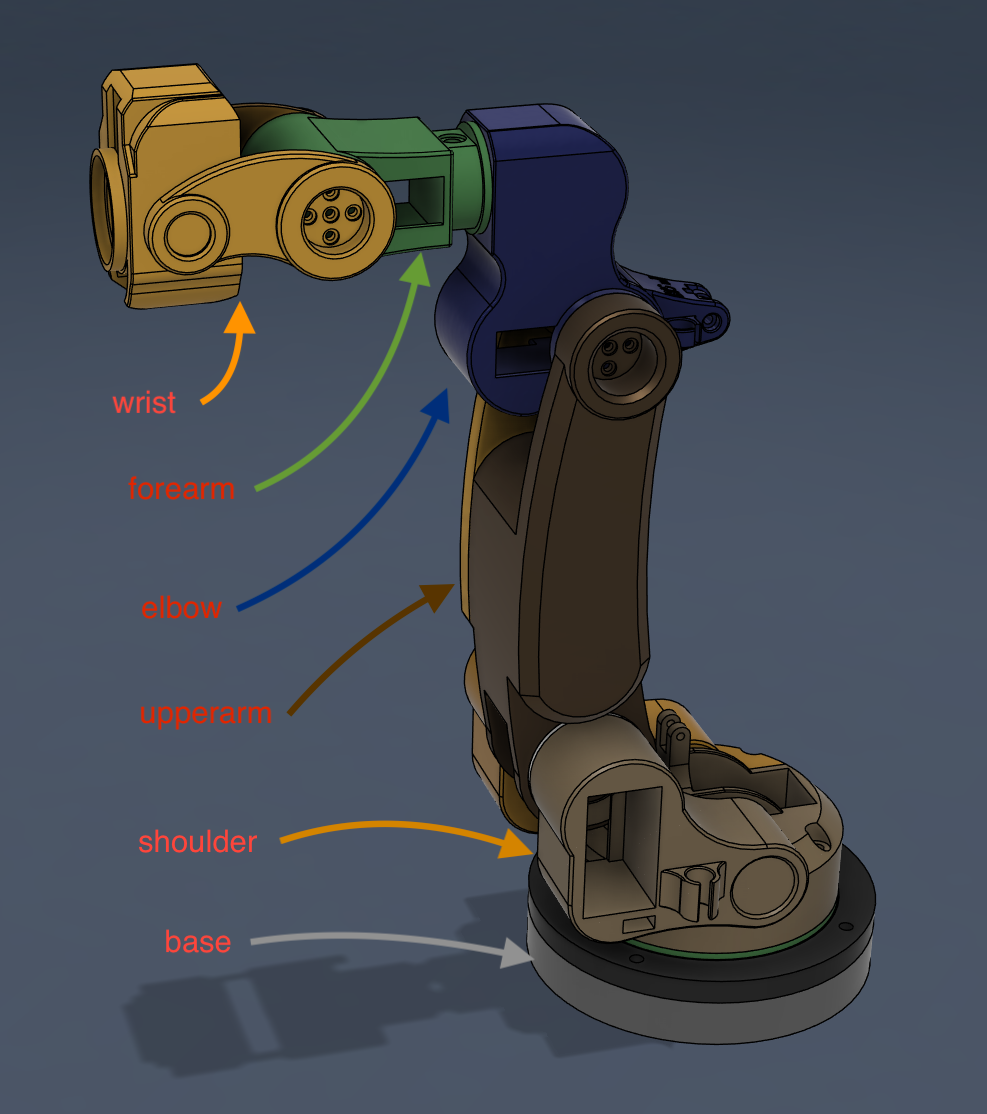
\includegraphics[width=0.65\linewidth]{images/arm_model.png}
    \caption{Model CAD sześcioosiowego ramienia manipulacyjnego z podziałem na główne człony kinematyczne}
    \label{fig:arm_model}
\end{figure}

Aby zapewnić płynność ruchu, zminimalizować luzy oraz bezpiecznie przenieść obciążenia statyczne i dynamiczne na strukturę nośną, wdrożono zróżnicowany system łożyskowania. W newralgicznym węźle łączącym podstawę z barkiem, narażonym na największe siły oraz momenty wywracające wynikające z maksymalnego wysięgu ramienia, zastosowano rozwiązanie hybrydowe. Składa się ono z szerokiego łożyska wieńcowego (typu \textit{lazy susan}) przenoszącego główne obciążenia osiowe oraz umieszczonego centralnie wewnątrz mechanizmu łożyska stożkowego. Pozostałe węzły kinematyczne ramienia zostały wyposażone w standardowe łożyska poprzeczne, co w zupełności wystarcza do poprawnego przenoszenia mniejszych obciążeń w wyższych partiach manipulatora.

Ostatnim ogniwem łańcucha kinematycznego jest efektor końcowy w postaci chwytaka dwuszczękowego. Model mechanizmu chwytającego zaprezentowano na rysunku \ref{fig:gripper_model}.

\begin{figure}[ht]
    \centering
    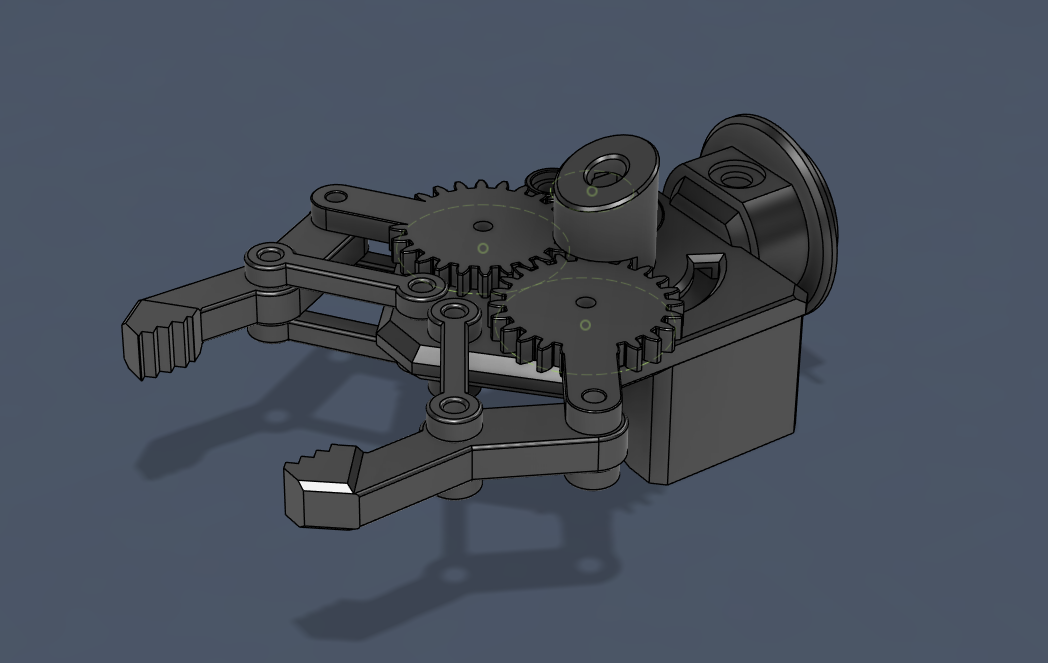
\includegraphics[width=0.75\linewidth]{images/gripper_model.png}
    \caption{Model CAD efektora końcowego wykorzystującego przekładnię zębatą do synchronizacji szczęk}
    \label{fig:gripper_model}
\end{figure}

Chwytak napędzany jest pojedynczym serwomechanizmem. Aby zapewnić równoległe i symetryczne zamykanie obu szczęk względem osi centralnej, w mechanizmie zintegrowano przekładnię zębatą. Zębatki sprzęgają ruch obu ramion chwytaka, co gwarantuje precyzyjne i powtarzalne centrowanie chwytanych obiektów, ułatwiając tym samym proces zautomatyzowanego planowania trajektorii.

\section{Dobór napędów i mechanizmy wspomagające}

Funkcję jednostek napędowych w zaprojektowanym manipulatorze pełnią inteligentne serwomechanizmy magistralowe ST3215 firmy Waveshare (rys. \ref{fig:st3215_servo}). Wybór tego konkretnego modelu podyktowany był przede wszystkim koniecznością zapewnienia bardzo wysokiego momentu obrotowego (wymaganego do poruszania wydrukowanymi członami ramienia) oraz możliwością pracy w zamkniętej pętli sprzężenia zwrotnego. Zastosowanie tak silnych napędów wiązało się jednak z koniecznym kompromisem projektowym. Ich stosunkowo duże gabaryty i masa własna wpłynęły na ostateczne rozmiary niektórych elementów układu, co jest szczególnie zauważalne w dość masywnej konstrukcji efektora końcowego (chwytaka). W całym systemie wykorzystano łącznie osiem takich aktuatorów.

\begin{figure}[ht]
    \centering
    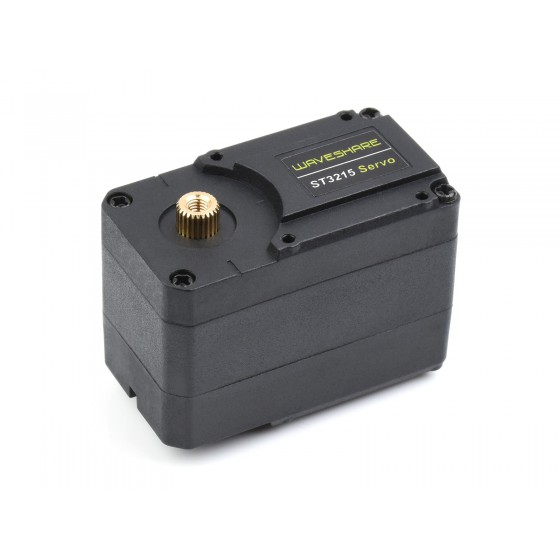
\includegraphics[width=0.55\linewidth]{images/st3215_servo.jpg}
    \caption{Serwomechanizm magistralowy ST3215 wykorzystany jako główny element napędowy ramienia}
    \label{fig:st3215_servo}
\end{figure}

Zastosowanie serwomechanizmów z interfejsem szeregowym pozwoliło na ich częściowe łączenie kaskadowe (ang. \textit{daisy-chaining}). Chociaż specyfika kinematyczna ramienia nadal wymagała doprowadzenia głównych linii zasilających i sygnałowych do kluczowych węzłów obrotowych, to możliwość szeregowego spięcia blisko sąsiadujących napędów pomogła ograniczyć całkowitą ilość i złożoność okablowania wewnątrz robota. Co najważniejsze, wbudowane w serwa mikrokontrolery umożliwiają ciągły odczyt parametrów telemetrycznych. System nadrzędny w czasie rzeczywistym monitoruje aktualną pozycję wału, napięcie zasilania, pobór prądu oraz temperaturę każdego z napędów, co stanowi podstawę dla wdrożenia mechanizmów bezpieczeństwa.

Z punktu widzenia kinematyki, ramię posiada sześć stopni swobody, jednak do realizacji ruchu wykorzystuje siedem silników (ósmy serwomechanizm odpowiada za napęd szczęk chwytaka). Z uwagi na fakt, że staw barkowy (\textit{shoulder}) jest elementem przenoszącym największe obciążenia statyczne i dynamiczne – wynikające z masy całego ramienia oraz ładunku – zastosowano w nim konfigurację podwójną. Dwa serwomechanizmy (lewy i prawy) zostały zamontowane przeciwsobnie na jednej osi obrotu i pracują w pełni synchronicznie. Rozwiązanie to pozwala na podwojenie sumarycznego momentu obrotowego dostępnego w tym krytycznym węźle.

Mimo zastosowania wydajnych napędów oraz podwójnego serwomechanizmu w barku, praca ramienia na maksymalnym wysięgu wiąże się ze znacznym wzrostem prądu trzymania (ang. \textit{holding current}), co mogłoby prowadzić do szybkiego przegrzewania się silników oraz drenażu akumulatora. Aby zniwelować to zjawisko, w konstrukcji zaimplementowano pasywny system kompensacji grawitacji. 

Mechanizm wspomagający składa się z wytrzymałej sprężyny naciągowej, zamocowanej pomiędzy obrotową podstawą a członem łokciowym manipulatora. Kluczowym elementem tego układu jest zastosowanie śruby rzymskiej, która pełni rolę płynnego regulatora napięcia wstępnego sprężyny. Odpowiednio skalibrowana sprężyna generuje moment siły przeciwny do momentu wywoływanego przez grawitację, działając jak fizyczna przeciwwaga. Dzięki temu systematycznie odciąża serwomechanizmy, pozwalając im na pracę z optymalną wydajnością prądową nawet w skrajnie rozciągniętych pozycjach manipulatora.

\section{Jednostka obliczeniowa, elektronika i sensoryka}

Realizacja założeń projektowych, w szczególności jednoczesna obsługa komunikacji bezprzewodowej, obliczanie kinematyki ramienia w czasie rzeczywistym oraz akwizycja strumienia wideo, wymagała zastosowania wydajnego komputera pokładowego. Jako główną jednostkę obliczeniową robota (ang. \textit{Controller Node}) wybrano mikrokomputer Raspberry Pi 5 wyposażony w 8 GB pamięci RAM. Architektura oparta na wielordzeniowym procesorze ARM zapewnia wystarczającą moc obliczeniową do płynnego zarządzania środowiskiem uruchomieniowym bazującym na języku Python oraz do utrzymania stabilnego opóźnienia sieciowego podczas strumieniowania danych do stacji operatorskiej.

Z uwagi na specyfikę cyfrowej magistrali szeregowej wykorzystywanej przez serwomechanizmy ST3215, bezpośrednie sterowanie nimi z poziomu styków GPIO mikrokomputera Raspberry Pi byłoby nieefektywne i podatne na błędy czasowe (tzw. \textit{jitter}). Z tego względu w architekturze elektroniki zastosowano dedykowany sterownik pośredniczący (ang. \textit{Servo Driver}) firmy Waveshare, którego centralnym elementem jest mikrokontroler z rodziny ESP32. Układ ten pełni funkcję sprzętowego interfejsu (mostka) pomiędzy wysokopoziomowymi poleceniami wysyłanymi z Raspberry Pi a niskopoziomowym protokołem komunikacyjnym magistrali serwomechanizmów. Rozwiązanie to odciąża główną jednostkę obliczeniową i gwarantuje wysoką niezawodność odczytu telemetrii.

Kluczowym elementem sensorycznym systemu, warunkującym poprawne działanie modułu sztucznej inteligencji, jest kamera pokładowa. Do akwizycji obrazu wykorzystano kamerę internetową A4Tech PK-910H, podłączoną do komputera Raspberry Pi za pomocą interfejsu USB. Wybór tego sensora podyktowany był koniecznością uzyskania zadowalającej ostrości obrazu (rozdzielczość 1080p) oraz odpowiedniego kąta widzenia przy zachowaniu pełnej kompatybilności ze środowiskiem systemu Linux (standard UVC -- \textit{USB Video Class}). 

Kamera została zamocowana na przedostatnim członie ramienia (przedramieniu), co pozwala na dynamiczną zmianę punktu widzenia w zależności od aktualnej pozycji manipulatora. Obraz pozyskiwany z sensora nie jest przetwarzany bezpośrednio na pokładzie robota – ze względu na wysokie zapotrzebowanie algorytmów wizyjnych na zasoby sprzętowe, surowy strumień wideo przesyłany jest siecią bezprzewodową do stacji operatorskiej (ang. \textit{Compute Node}), gdzie poddawany jest docelowej analizie przez model detekcji obiektów.

\section{Architektura zasilania i układ zabezpieczeń}

Zapewnienie stabilnego i bezpiecznego zasilania dla układów o dużym, impulsowym poborze prądu stanowiło jedno z głównych wyzwań integracyjnych. Zgodnie z przyjętą architekturą izolowaną, układ ramienia oraz jednostka obliczeniowa zasilane są z niezależnego akumulatora litowo-polimerowego (LiPo) w konfiguracji 3S (trzy ogniwa połączone szeregowo). Pakiet ten dostarcza napięcie nominalne na poziomie 11,1 V, co stanowi wartość optymalną do zasilania wysokonapięciowych serwomechanizmów ST3215.

W celu zagwarantowania bezpieczeństwa, główna linia zasilająca (+VCC) została natychmiast za akumulatorem zabezpieczona szybkim bezpiecznikiem samochodowym o wartości 15 A. Prąd o takim natężeniu pozwala na bezproblemową, jednoczesną pracę wszystkich ośmiu serwomechanizmów pod obciążeniem oraz mikrokomputera. Bezpośrednio za bezpiecznikiem umieszczono główny włącznik kołyskowy. Z uwagi na zintegrowane w nim podświetlenie LED, do włącznika doprowadzono również główny przewód masy (GND).

Aby uniknąć zjawiska skumulowanego spadku napięcia na cienkich przewodach, wdrożono scentralizowany system dystrybucji zasilania. Opiera się on na szybkozłączkach instalacyjnych typu Wago, które umieszczono w dolnej części bazy, tuż za włącznikiem. Pozwoliło to na podział głównej szyny prądowej na dedykowane sekcje zasilające:
\begin{itemize}
    \item \textbf{Sekcja 1:} zasila serwomechanizm nr 1 (obrót bazy),
    \item \textbf{Sekcja 2:} zasila serwomechanizmy nr 2 i 3 (podwójny napęd stawu barkowego),
    \item \textbf{Sekcja 3:} zasila serwomechanizmy nr 4 i 5 (ramię i łokieć),
    \item \textbf{Sekcja 4:} zasila serwomechanizmy nr 6, 7 i 8 (przedramię, nadgarstek i chwytak).
\end{itemize}

Wewnątrz wyżej wymienionych grup zasilanie prowadzone jest kaskadowo, co stanowi optymalny kompromis pomiędzy ilością okablowania a stabilnością napięcia. Warto zaznaczyć, że sterownik serwomechanizmów (Servo Driver) nie pobiera energii z głównej szyny zasilającej LiPo -- jest on zasilany niezależnie poprzez złącze USB. Aby jednak zapewnić prawidłową propagację sygnałów logicznych, przewód masy (GND) sterownika został połączony z głównym blokiem dystrybucyjnym Wago, tworząc wspólną masę dla całej instalacji. Linia sygnałowa magistrali (DATA) wychodząca z kontrolera ESP32 nie jest prowadzona ściśle kaskadowo przez wszystkie napędy. Z uwagi na ułatwienie poprowadzenia przewodów wewnątrz ramienia, zastosowano architekturę mieszaną z rozgałęzieniami, w której główna szyna danych dzieli się na odnogi doprowadzone do poszczególnych sekcji.

Ostatnia linia zasilająca wyprowadzona z kostki Wago dedykowana jest dla jednostki obliczeniowej. Napięcie z akumulatora LiPo przekazywane jest na moduł przetwornicy obniżającej (ang. \textit{step-down buck converter}), która stabilizuje napięcie do poziomu 5 V, doprowadzanego następnie złączem USB-C do mikrokomputera Raspberry Pi 5. Uproszczony schemat blokowy opisanej topologii zasilania i komunikacji przedstawiono na rysunku \ref{fig:power_schematic}.

\begin{figure}[H]
    \centering
    \resizebox{\textwidth}{!}{
    \begin{tikzpicture}[
        node distance=1.5cm and 2cm,
        box/.style={draw, rectangle, rounded corners=2pt, minimum width=3.5cm, minimum height=1cm, align=center, font=\small},
        wago/.style={draw, rectangle, rounded corners=4pt, fill=gray!15, minimum width=13.5cm, minimum height=1cm, align=center, font=\small\bfseries},
        vcc/.style={draw, red, -{Latex}, thick},
        gnd/.style={draw, black, -{Latex}, thick},
        data/.style={draw, blue, dashed, -{Latex}, thick},
        usb/.style={draw, purple, -{Latex}, thick}
    ]

    % --- POZIOM 1 (GÓRA) ---
    \node[box] (switch) {Włącznik z LED};
    \node[box, left=2.5cm of switch] (lipo) {Akumulator LiPo 3S \\ (11.1 V)};
    \node[box, right=2.5cm of switch] (fuse) {Bezpiecznik \\ (15 A)};

    % --- POZIOM 2 ---
    \node[wago, below=1.5cm of switch] (wago) {Centralny Blok Dystrybucyjny};

    % --- POZIOM 3 ---
    \node[box, below=1.5cm of wago] (driver) {Servo Driver \\ (ESP32)};
    \node[box, left=2.5cm of driver] (stepdown) {Przetwornica \\ Step-Down (5 V)};

    % --- POZIOM 4 (DÓŁ) ---
    \node[box, below=2.5cm of stepdown] (rpi) {Raspberry Pi 5};
    \node[box] (servos) at (fuse |- rpi) {Sekcje Serwomechanizmów \\ (1 do 8)};

    % ==========================================
    % POŁĄCZENIA
    % ==========================================

    % 1. LiPo -> Włącznik -> Bezpiecznik
    \draw[vcc] (lipo) -- (switch) node[midway, above, text=red, font=\footnotesize] {+VCC};
    \draw[vcc] (switch) -- (fuse);

    % 2. Bezpiecznik -> WAGO (Pionowo w dół)
    \draw[vcc] (fuse.south) -- (fuse.south |- wago.north) node[pos=0.5, right, text=red, font=\footnotesize] {+VCC};

    % 3. Masa (GND): LiPo -> WAGO, oraz WAGO -> Włącznik (LED)
    \draw[gnd] (lipo.south) -- (lipo.south |- wago.north) node[pos=0.5, left, font=\footnotesize] {GND};
    \draw[gnd] (switch.south |- wago.north) -- (switch.south) node[midway, right, font=\footnotesize] {GND};

    % 4. WAGO -> Step-Down (Lewa kolumna)
    \draw[vcc] ([xshift=-15pt]wago.south -| stepdown.north) -- ([xshift=-15pt]stepdown.north) node[pos=0.5, left, text=red, font=\footnotesize] {+VCC};
    \draw[gnd] ([xshift=15pt]wago.south -| stepdown.north) -- ([xshift=15pt]stepdown.north) node[pos=0.5, right, font=\footnotesize] {GND};

    % 5. Step-Down -> Raspberry Pi (Lewa kolumna)
    \draw[vcc] ([xshift=-15pt]stepdown.south) -- ([xshift=-15pt]rpi.north) node[pos=0.5, left, text=red, font=\footnotesize] {5V};
    \draw[gnd] ([xshift=15pt]stepdown.south) -- ([xshift=15pt]rpi.north) node[pos=0.5, right, font=\footnotesize] {GND};

    % 6. WAGO -> Servo Driver (Środek)
    \draw[gnd] (wago.south) -- (driver.north) node[pos=0.5, right, font=\footnotesize] {Wspólna Masa (GND)};

    % 7. WAGO -> Serwomechanizmy (Prawa kolumna)
    \draw[vcc] ([xshift=-15pt]wago.south -| servos.north) -- ([xshift=-15pt]servos.north) node[pos=0.7, left, text=red, font=\footnotesize] {+VCC};
    \draw[gnd] ([xshift=15pt]wago.south -| servos.north) -- ([xshift=15pt]servos.north) node[pos=0.7, right, font=\footnotesize] {GND};

    % 8. Servo Driver -> Serwomechanizmy (Linia Danych - tekst przesunięty w prawo)
    \draw[data] (driver.east) -- ++(1.5,0) node[pos=0.7, above, text=blue, font=\footnotesize] {Linia Danych} |- (servos.west);

    % 9. Raspberry Pi -> Servo Driver (Tekst rozdzielony góra/dół)
    \draw[usb] (rpi.east) -| (driver.south) node[pos=0.25, above, text=purple, font=\footnotesize] {USB-A $\rightarrow$ USB-C} node[pos=0.25, below, text=purple, font=\footnotesize] {(Zasilanie + Dane)};

    \end{tikzpicture}
    }
    \caption{Schemat blokowy dystrybucji zasilania i komunikacji magistrali szeregowej}
    \label{fig:power_schematic}
\end{figure}

\section{Integracja mechaniczna systemu i zarządzanie okablowaniem}

Ostatnim etapem budowy warstwy sprzętowej była fizyczna integracja wszystkich opisanych wcześniej podsystemów w jedną, spójną jednostkę mobilną. W celu optymalizacji dostępnej przestrzeni oraz ułatwienia obsługi serwisowej robota, wprowadzono autorskie modyfikacje mechaniczne platformy bazowej. Na rysunku \ref{fig:ugv_extender} zaprezentowano model CAD zintegrowanego modułu rozszerzającego. Kolorem zielonym oznaczono górną płaszczyznę platformy UGV02, do której przytwierdzone są fabryczne szyny montażowe (kolor niebieski). W szyny te wsunięto specjalnie zaprojektowane i wydrukowane w technologii 3D adaptery nośne (kolor czerwony). Stanowią one solidne punkty mocowania dla dodatkowego, aluminiowego pokładu (kolor żółty), dostarczanego jako opcjonalne wyposażenie podwozia.

\begin{figure}[H]
    \centering
    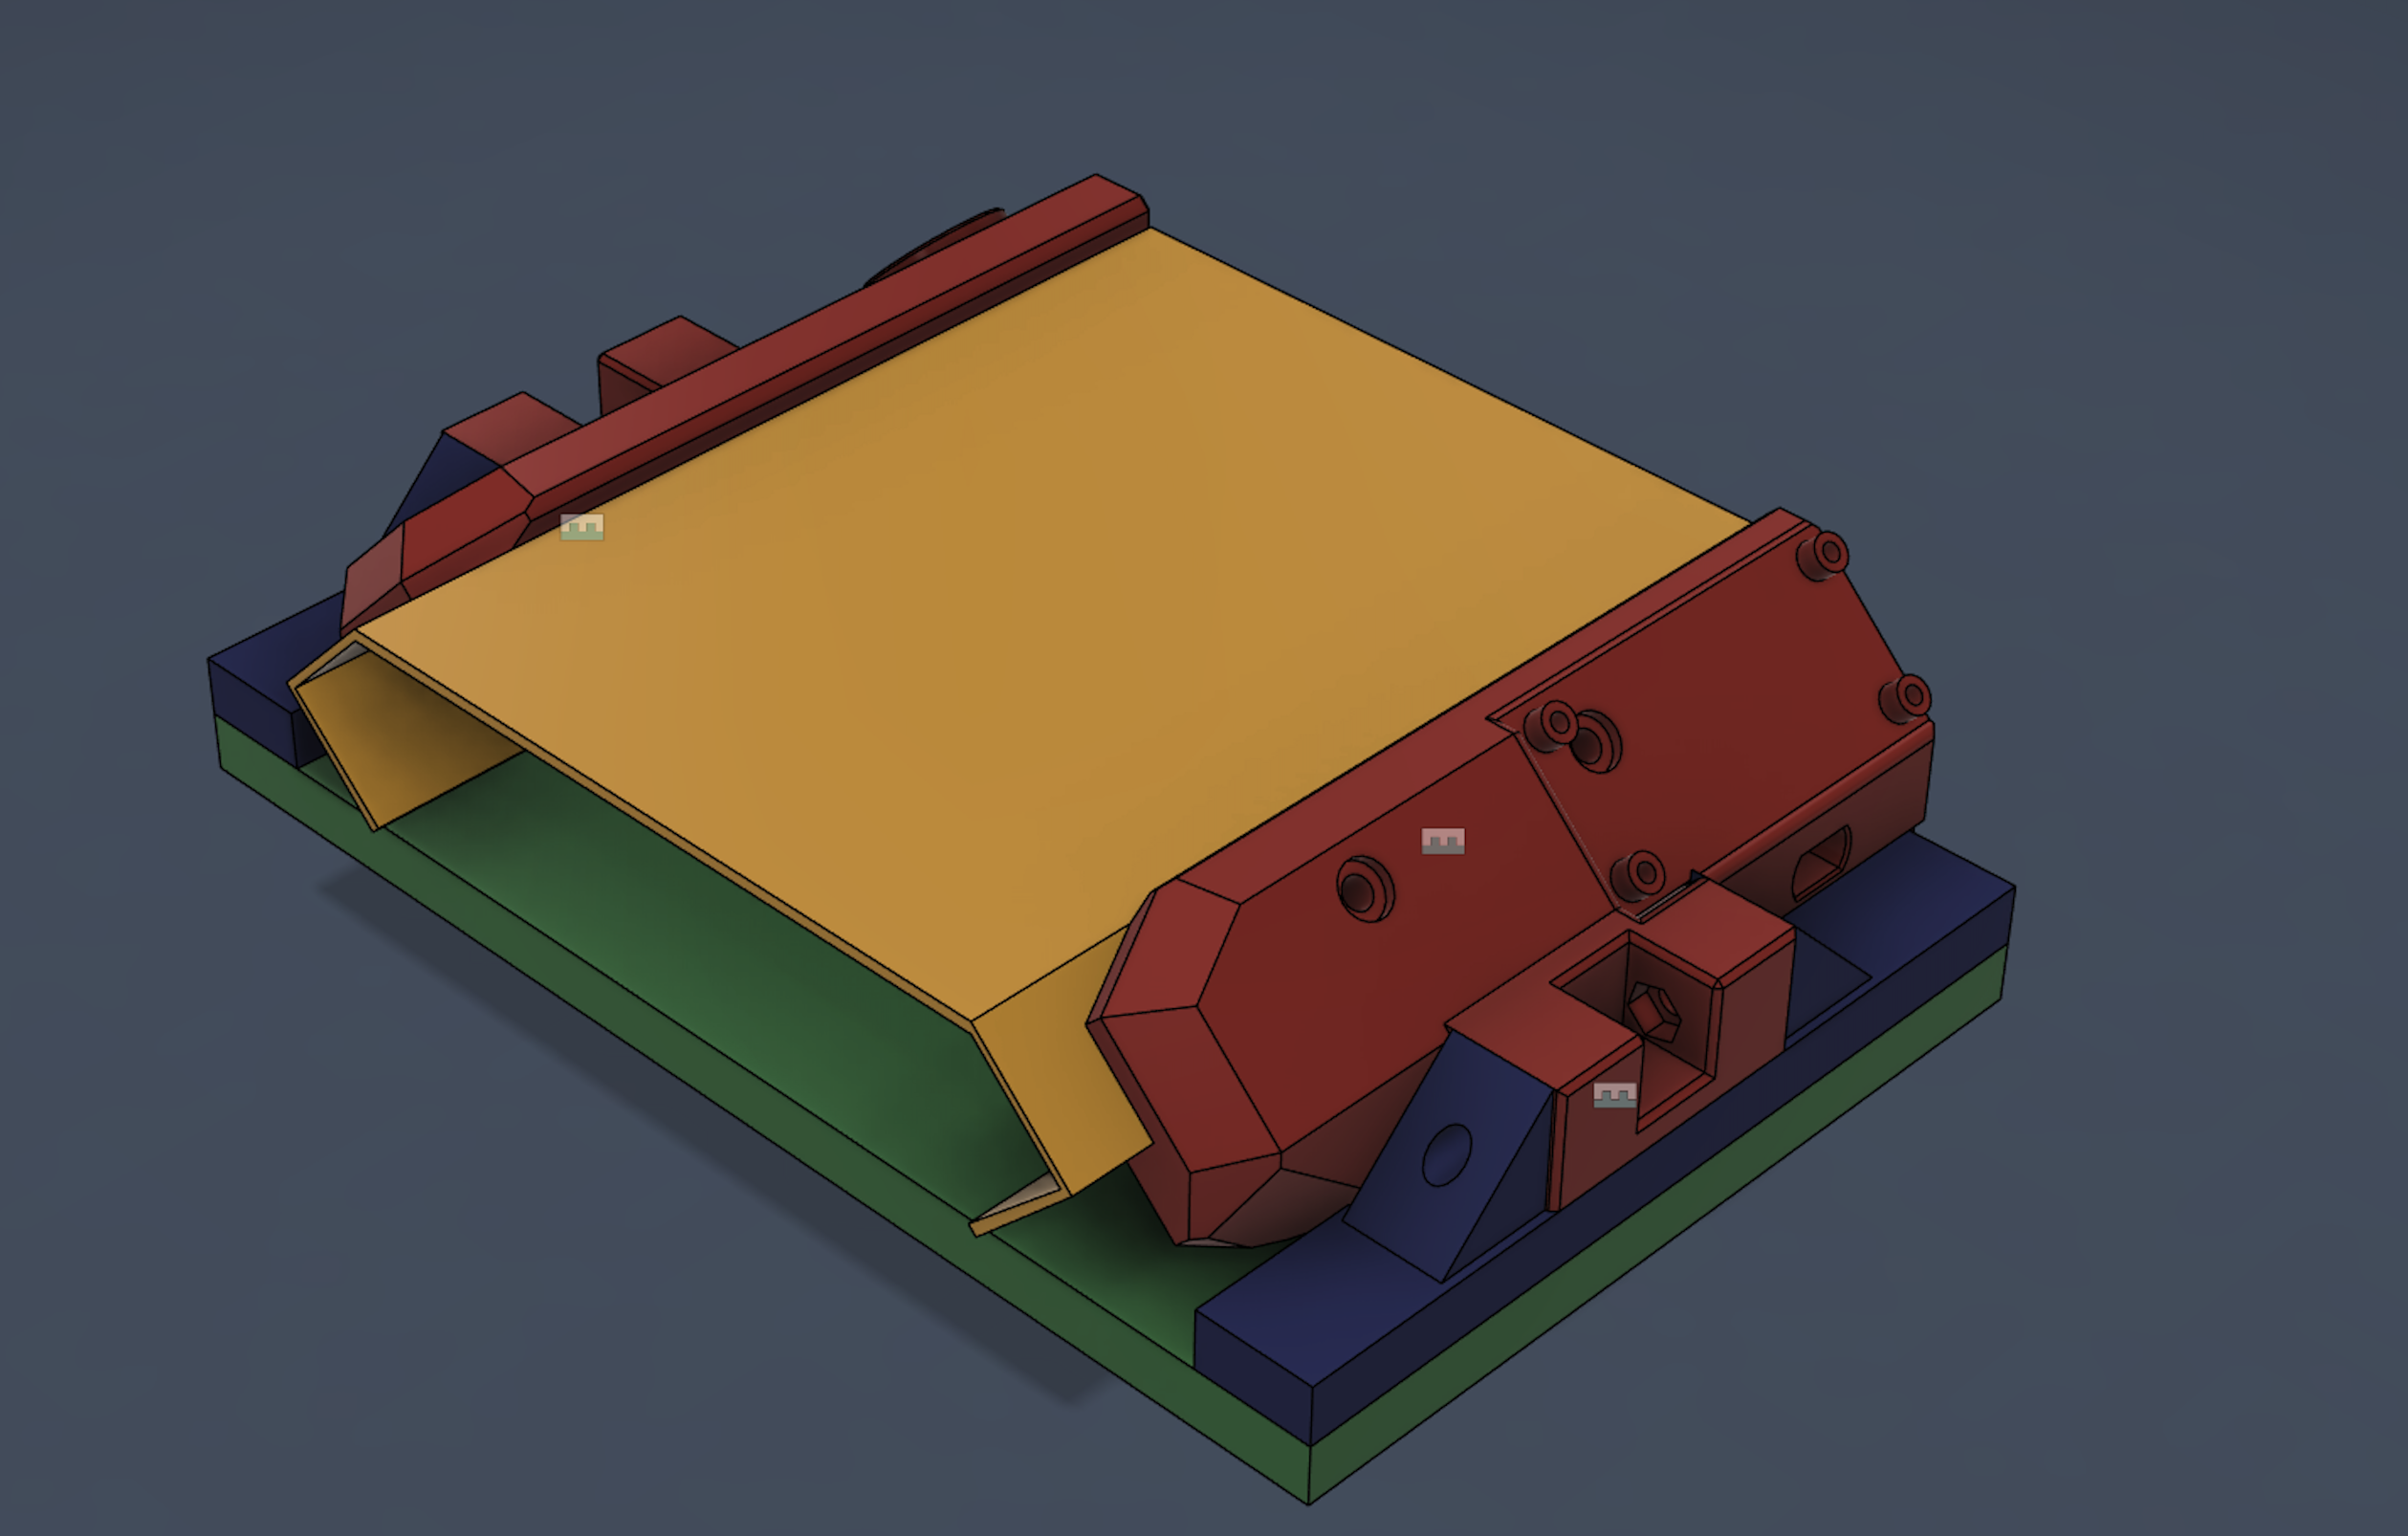
\includegraphics[width=0.75\linewidth]{images/ugv_extender.png}
    \caption{Model CAD modułu rozszerzającego: zielony -- pokrywa bazy, niebieski -- szyny, czerwony -- adaptery 3D, żółty -- pokład aluminiowy}
    \label{fig:ugv_extender}
\end{figure}

Kluczową zaletą zaprojektowanego mechanizmu jest możliwość płynnego przesuwania całego zmontowanego modułu wzdłuż szyn, równolegle do osi podłużnej robota. Takie rozwiązanie konstrukcyjne gwarantuje bezproblemowy i szybki dostęp do włącznika zasilania platformy UGV02, fabrycznego gniazda ładowania bazy jezdnej, a także do złączy zasilających głównego akumulatora LiPo zasilającego ramię. Pozwala to na wygodne podłączenie ładowarki bez konieczności kłopotliwego demontażu ramienia manipulacyjnego lub innych elementów konstrukcyjnych.

Dodatkowy górny pokład posłużył do ergonomicznego rozmieszczenia elektroniki, w tym w szczególności sterownika serwomechanizmów (Servo Driver) firmy Waveshare opartego na mikrokontrolerze ESP32. W celu zapewnienia wysokiej niezawodności i ochrony okablowania przed przetarciami w trakcie ruchu ramienia, wszystkie główne wiązki przewodów zostały poprowadzone w elastycznych oplotach ochronnych. Zastosowanie oplotów ułatwiło segregację linii sygnałowych i zasilających, znacząco podnosząc bezpieczeństwo przeciwzwarciowe oraz ogólną estetykę i niezawodność układu.


% =========================================================================
% ROZDZIAŁ 5
% =========================================================================
\chapter{Architektura systemu sterowania i komunikacja}

Współczesne systemy robotyczne, szczególnie te integrujące algorytmy sztucznej inteligencji z fizycznymi układami wykonawczymi, wymagają starannie zaprojektowanej architektury oprogramowania. Głównym wyzwaniem w takich projektach jest zapewnienie płynnej i szybkiej wymiany danych pomiędzy warstwą percepcyjną, modułem sterującym oraz sprzętowymi kontrolerami napędów. Niniejszy rozdział opisuje strukturę logiczną stworzonego systemu, podział ról pomiędzy jednostkami obliczeniowymi oraz zastosowane technologie komunikacyjne.

\section{Logiczny podział ról w architekturze rozproszonej}

Zastosowanie zaawansowanych modeli głębokich sieci neuronowych (takich jak algorytm YOLO) do analizy obrazu w czasie rzeczywistym wymaga znacznych zasobów obliczeniowych, w szczególności dostępu do wydajnych akceleratorów. Z tego względu w projekcie zrezygnowano ze scentralizowanego przetwarzania wszystkich danych wyłącznie na pokładzie robota. Zamiast tego wdrożono architekturę systemu rozproszonego. Jak zauważa się w literaturze przedmiotu, przeniesienie złożonych obliczeniowo zadań z mobilnych jednostek o ograniczonym budżecie energetycznym na zewnętrzne stacje robocze pozwala na sprawniejszą realizację algorytmów percepcji, znacząco zwiększając możliwości poznawcze układów zrobotyzowanych \cite{siegwart2011introduction}.

W zaprojektowanym systemie wydzielono dwa główne węzły (ang. \textit{nodes}), z których każdy pełni ściśle określoną funkcję:

\begin{itemize}
    \item \textbf{Węzeł obliczeniowy (ang. \textit{Compute Node}) -- Stacja operatorska:}
    Stanowi centrum percepcyjne i nadrzędny interfejs sterujący całego systemu. Rolę tę pełni zewnętrzny komputer (laptop) wyposażony w środowisko zdolne do szybkiej inferencji modelu detekcji obiektów. Jednostka ta odbiera surowy strumień wideo z robota i w czasie rzeczywistym poddaje go analizie wizyjnej, lokalizując docelowe obiekty w kadrze poprzez wyznaczanie i wizualizację ramek ograniczających (ang. \textit{bounding boxes}). Równolegle, stacja operatorska służy do generowania i wysyłania wysokopoziomowych danych sterujących (np. współrzędnych docelowych) do robota.
    
    \item \textbf{Węzeł sterujący (ang. \textit{Controller Node}) -- Jednostka pokładowa:}
    Zadanie to realizowane jest przez mikrokomputer Raspberry Pi 5 znajdujący się fizycznie na platformie jezdnej. Do jego głównych zadań należy nieprzerwana akwizycja obrazu z kamery USB i strumieniowanie go przez sieć Wi-Fi do stacji operatorskiej. Równolegle jednostka ta odbiera wysokopoziomowe komendy ruchu. Wykorzystując zaimplementowany algorytm analitycznej kinematyki odwrotnej (ang. \textit{Inverse Kinematics} -- IK), Raspberry Pi przelicza otrzymane dane na docelowe kąty obrotu dla poszczególnych stawów ramienia. Z uwagi na analityczny (równaniowy) charakter modelu, obliczenia te są wysoce zoptymalizowane i realizowane w ułamku sekundy, nie obciążając znacząco procesora. Następnie wyliczone pozycje przekazywane są interfejsem szeregowym do sterownika ESP32 (Servo Driver), który realizuje ruch napędów.
\end{itemize}

Taki ścisły podział kompetencji niesie za sobą wymierne korzyści inżynierskie. Odciąża procesor jednostki pokładowej z zadań wizyjnych, pozwalając mu skupić się na obliczeniach kinematycznych i utrzymaniu stabilnej komunikacji. Jednocześnie zapewnia elastyczność – stację operatorską można w dowolnym momencie zmodernizować w celu uzyskania szybszej inferencji AI, bez konieczności ingerencji w sprzęt i oprogramowanie samego robota.

\section{Topologia sieci i protokoły komunikacyjne}

Zapewnienie stabilnej, asynchronicznej i niskopoziomowej wymiany danych między stacją operatorską a robotem jest zadaniem krytycznym z punktu widzenia płynności sterowania. Zamiast tradycyjnego modelu opartego na surowych gniazdach TCP/UDP, w projekcie wdrożono wydajną bibliotekę asynchronicznego przesyłania wiadomości \textit{ZeroMQ} (ZMQ). Rozwiązanie to warunkuje wysoką przepustowość, automatyczne zarządzanie retransmisją oraz oferuje wbudowane wzorce komunikacyjne, co stanowi standard w nowoczesnych, rozproszonych systemach robotycznych.

Fizyczną warstwę transportową stanowi standardowa sieć bezprzewodowa Wi-Fi (IEEE 802.11). Mikrokomputer Raspberry Pi pobiera swój lokalny adres IP i wyświetla go na module OLED, co umożliwia stacji bazowej nawiązanie bezpośredniego połączenia. Z punktu widzenia oprogramowania, zewnętrzna topologia sieciowa została podzielona na trzy niezależne, równoległe kanały komunikacyjne (strumienie), z których każdy operuje na dedykowanym porcie i wykorzystuje zoptymalizowany wzorzec przesyłu danych:

\begin{enumerate}
    \item \textbf{Strumień Sterowania (Port 5555):} 
    Odpowiada za przesyłanie poleceń ruchowych z węzła obliczeniowego do jednostki pokładowej. Zrealizowany jest w oparciu o wzorzec Żądanie-Odpowiedź (ang. \textit{Request-Reply}). Stacja bazowa (klient) cyklicznie wysyła pakiety w formacie JSON, zawierające m.in. aktualny stan kontrolera (gamepada) oraz wyliczone współrzędne docelowe. Główna usługa na robocie (ang. \textit{Arm Service}) odbiera pakiet, aplikuje go do równań kinematyki, a następnie odsyła potwierdzenie, zamykając cykl.

    \item \textbf{Strumień Wideo (Port 5556):}
    Dedykowany wyłącznie do transmisji obrazu z pokładowej kamery USB. Działa w oparciu o wzorzec Publikuj-Subskrybuj (ang. \textit{Publish-Subscribe}). Skrypt na Raspberry Pi przechwytuje klatki, dokonuje ich natychmiastowej kompresji do formatu JPEG za pomocą biblioteki OpenCV, a następnie publikuje surowe ciągi bajtów. Aby zminimalizować zjawisko opóźnienia wizyjnego (ang. \textit{latency}), po stronie subskrybenta (laptopa) aktywowano sprzętową opcję \texttt{ZMQ\_CONFLATE}. Powoduje ona ignorowanie starszych, zalegających w buforze klatek wideo na rzecz przetwarzania wyłącznie tej najnowszej.
    
    \item \textbf{Strumień Telemetrii (Port 5557):}
    Działa analogicznie do strumienia wideo (wzorzec PUB/SUB), przesyłając z robota do laptopa struktury danych JSON. Pakiety te zawierają zbiór krytycznych informacji diagnostycznych zebranych w czasie rzeczywistym, takich jak: napięcie głównego zasilania akumulatorowego, temperatury i prądy poszczególnych serwomechanizmów, aktualne kąty w stawach oraz logi systemowe.
\end{enumerate}

Warto zaznaczyć, że biblioteka ZeroMQ została wykorzystana nie tylko do komunikacji zewnętrznej, ale również wewnątrz samego środowiska robota. W celu separacji logicznej modułów, zarządzanie ramieniem oraz platformą jezdną rozdzielono na niezależne procesy (\textit{Arm Service} oraz \textit{Chassis Service}). Komunikują się one ze sobą lokalnie poprzez dedykowane, wewnętrzne porty (5558 i 5559), tworząc bezpieczną i odporną na błędy architekturę mikrousług (ang. \textit{microservices}).

\section{Architektura wieloprocesowa i nadzorca systemu (Supervisor)}

Implementacja złożonego systemu zrobotyzowanego w środowisku języka Python wiąże się z koniecznością ominięcia ograniczeń wynikających z globalnej blokady interpretera (ang. \textit{Global Interpreter Lock} -- GIL). Wykonywanie intensywnych operacji wejścia/wyjścia (takich jak akwizycja wideo), ciągłe nasłuchiwanie portów sieciowych oraz przeliczanie kinematyki w pojedynczym procesie doprowadziłoby do znacznych opóźnień i utraty płynności sterowania. Z tego względu na pokładzie jednostki \textit{Controller Node} wdrożono architekturę wieloprocesową z centralnym węzłem zarządzającym.

Główny skrypt startowy robota (\texttt{controller\_main.py}) nie realizuje bezpośrednio żadnych zadań percepcyjnych ani wykonawczych. Pełni on wyłącznie funkcję systemowego nadzorcy (ang. \textit{Process Supervisor}). Do jego zadań należy asynchroniczne uruchomienie i monitorowanie trzech kluczowych, niezależnych podprocesów:
\begin{itemize}
    \item \textbf{Arm Service:} moduł odpowiedzialny za komunikację ZMQ ze stacją bazową, obliczanie kinematyki oraz wysterowanie sterownika ESP32 ramienia.
    \item \textbf{Camera Service:} moduł dedykowany wyłącznie do sprzętowej akwizycji klatek obrazu z interfejsu USB, ich kompresji oraz strumieniowania w sieć.
    \item \textbf{Chassis Service:} moduł zarządzający komunikacją szeregową z mikrokontrolerem platformy jezdnej UGV02.
\end{itemize}

Takie podejście architektoniczne gwarantuje ścisłą izolację błędów (ang. \textit{fault isolation}). Awaria lub chwilowe zawieszenie się procesu obsługującego kamerę nie wpływa w żaden sposób na proces obliczający kinematykę ramienia, co pozwala na zachowanie ciągłości sterowania fizycznego.

Co więcej, nadzorca systemu implementuje deterministyczny mechanizm reagowania na awarie krytyczne. W głównej pętli programu nieustannie weryfikowany jest status cyklu życia wszystkich uruchomionych podprocesów (metoda \texttt{poll()}). W przypadku wykrycia niespodziewanego zakończenia pracy któregokolwiek z serwisów (np. z powodu rozłączenia fizycznego przewodu), nadzorca natychmiastowo inicjuje procedurę awaryjnego zatrzymania systemu (ang. \textit{emergency shutdown}). Polega ona na bezpiecznym wysłaniu sygnałów terminacji (SIGTERM) do pozostałych działających modułów oraz poprawnym zamknięciu współdzielonego pliku logów (\texttt{robot.log}), który gromadzi diagnostyczne wyjścia standardowe (stdout/stderr) ze wszystkich podprocesów.

Zastosowanie architektury wieloprocesowej nadzorowanej przez nadrzędny skrypt kontrolny sprawia, że oprogramowanie robota jest nie tylko wydajne i wolne od blokad (ang. \textit{non-blocking}), ale przede wszystkim wysoce odporne na błędy, co stanowi fundamentalny wymóg w projektowaniu nowoczesnej robotyki mobilnej.


 % =========================================================================
% ROZDZIAŁ 6 - Zmieniony profil na czysty kod robota (Raspberry + ESP32)
% =========================================================================
\chapter{Oprogramowanie pokładowe robota}
\section{Sterownik serwomechanizmów i odczyt telemetrii z magistrali} % tu opiszemy serial_link.py
\section{Implementacja kinematyki analitycznej manipulatora} % tu opiszemy wzory i IK
\section{Ograniczenia przestrzeni roboczej i sprzętowe limity bezpieczeństwa} % tu przeniesiemy MAX_REACH i JOINT_LIMITS
\section{Akwizycja i kompresja strumienia wideo z kamery pokładowej} % tu opiszemy camera_service.py
\section{Sterowanie platformą jezdną} % tu opiszemy chassis_service.py

% =========================================================================
% ROZDZIAŁ 7 - Idealnie zdefiniowany
% =========================================================================
\chapter{Implementacja modułu sztucznej inteligencji}
\section{Przygotowanie i konfiguracja modelu detekcji YOLO}
\section{Przetwarzanie obrazu w czasie rzeczywistym i augmentacja danych}

\addtocontents{toc}{\protect\newpage}

% =========================================================================
% ROZDZIAŁ 8 - Skupiony w 100% na aplikacji na PC (PySide6)
% =========================================================================
\chapter{Stworzenie stacji operatorskiej}
\section{Projekt graficznego interfejsu użytkownika (GUI)}
\section{Integracja bezprzewodowego kontrolera i mapowanie przycisków}
\section{Wizualizacja telemetrii i synchronizacja danych} % połączone logowanie i wideo

% =========================================================================
% ROZDZIAŁ 9 - Skupiony na testowaniu działania całości
% =========================================================================
\chapter{Testy funkcjonalne i weryfikacja systemu}
\section{Weryfikacja działania układu jezdnego}
\section{Testy kinematyki ramienia i precyzji manipulacji}
\section{Ewaluacja wydajności sieciowej i opóźnień (latency)} % Lepsze niż "mechanizmy bezp.", zbadamy tu działanie ZMQ
\section{Skuteczność algorytmów rozpoznawania obrazu}

% =========================================================================
% ROZDZIAŁ 10
% =========================================================================
\chapter{Wnioski i kierunki dalszego rozwoju}


% =========================================================================
% BIBLIOGRAFIA I PODSUMOWANIE ANGIELSKIE
% =========================================================================
\printbibliography[title={Literatura}]

\begingroup
\titleformat{\chapter}[hang]
  {\normalfont\fontsize{16}{20}\bfseries\centering}
  {\thechapter.}{1em}{}
      \clearpage
    \phantomsection

\addcontentsline{toc}{chapter}{Summary}
\chapter*{Summary}                            
\endgroup

\end{document}